
\section{Orbital Elements} \label{sec:orb} 
In astrodynamics, the osculating orbit of an object in space (at a given moment of time) is the gravitational Kepler orbit (i.e. ellipse or other conic) that it would have about its central body (corresponding to its actual position and velocity for that given moment of time) if perturbations were not present, see Vallado \cite{Vallado}.

An osculating orbit and the object's position upon it can be fully described by the six standard Keplerian orbital elements (osculating elements), which are easy to calculate as long as one knows the object's position and velocity relative to the central body. The osculating elements would remain constant in the absence of perturbations. However, real astronomical orbits experience perturbations that cause the osculating elements to evolve, sometimes very quickly. In cases where general celestial mechanical analysis of the motion have been carried out (as they have been for the major planets, the Moon, and other planetary satellites), the orbit can be described by a set of mean elements with secular and periodic terms. In the case of minor planets, a system of proper orbital elements has been devised to enable representation of the most important aspects of their orbits.

\textbf{Coordinate Frame:} Quasi-Inertial\\
Base coordinate frame is ICRF as describe in section \ref{sec:gen}.

\begin{itemize}
\item a - is the instantaneous semimajor axis of the orbit.
\item e - is the instantaneous eccentricity of the orbit.
\item i - the inclination of the orbital plane, is the instantaneous angle between the mean inertial north polar axis and the orbital angular momentum vector.
\item $\Omega$ - the right ascension of the ascending node, is the angle measured
eastward from the vernal equinox along the equator to that intersection with
the orbit plane where the vehicle passes from south to north. In the case
where inclination equals zero, the ascending node is defined to be the
X axis of the inertial reference system.
\item $\omega$ -  the argument of perigee, is the angle measured in the orbit plane between the ascending node and perigee, positive in the direction of travel in the orbit. In the case where eccentricity equals zero, perigee is defined to be at the ascending node.
\item $\theta$ the true anomaly, is the geocentric angular displacement of the vehicle measured from perigee in the orbit plane, and positive in the direction of travel in the orbit.
\end{itemize}


\begin{figure}[htp]
\centering
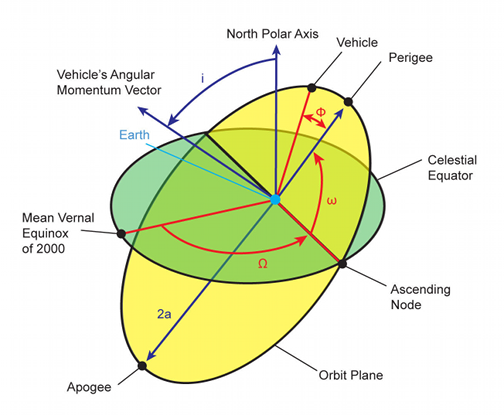
\includegraphics [width=7in]{figs/fig8.png}
\caption{Orbital Elements}
\label{fig:8}
\end{figure}

\subsection{Example Orbital Elements}
See the following JEOD models for an example, \hypermodelref{ORBITALELEMENTS} and \hypermodelref{DERIVEDSTATE}.


